\section{Macchina a stati finiti}
Il firmware implementato è stato formalizzato tramite una macchina a stati finiti (FSM). Un'automa a stati finiti è un modello matematico con cui è possibile descrivere in modo preciso e sintetico il comportamento di un sistema tramite un numero finito di stati, che rappresentano le condizioni operative nelle quali esso si può trovare. Il passaggio da uno stato all'altro avviene in seguito al verificarsi di particolari eventi e condizioni, che definiscono le \textit{funzioni di transizione}. Una caratteristica fondamentale delle FSM è rappresentata dalla necessità di garantire l'unicità dello stato che in un certo istante di tempo è attivo\todo{da rileggere}. Per questo motivo, è sempre possibile sapere con esattezza lo stato in cui si trova la macchina. Inoltre, è consentito effettuare solo una transizione alla volta. Le transizioni possibili da un particolare stato devono quindi essere mutuamente esclusive.
L'utilizzo di una macchina a numero finito di stai può essere adatto sia per la progettazione di un sistema sia per la descrizione di uno esistente. In particolare, è possibile modellare sistemi che sono:
\begin{itemize}
	\item dinamici, che quindi evolvono cambiando stato nel tempo;
	\item discreti, cioè che le variabili in ingresso e gli stati del sistema si possono rappresentare con valori discreti;
	\item a simboli finiti, cioè che il numero di variabili in ingresso e gli stati può essere espresso con un numeri finito;
\end{itemize}
Una macchina a stati può essere rappresentata attraverso un grafo, in cui i nodi identificano gli stati e gli archi rappresentano le transizioni causate da eventi. 

Il firmware realizzato per questo progetto è stato implementato, con le opportune modifiche, sia per l'acquisizione dei dati con il sensore MAX86916 sia con l'integrato MAXM86161. Sono stati identificati i seguenti stati:
\begin{enumerate}
	\setcounter{enumi}{-1}
	\item Start-up
	\item Idle
	\item Stream
	\item Error
\end{enumerate}
Nella figura \ref{fig:FSM} è stato riportato il grafico che riassume il comportamento della macchina a stati implementata.
\begin{figure}[b]
	\centering
	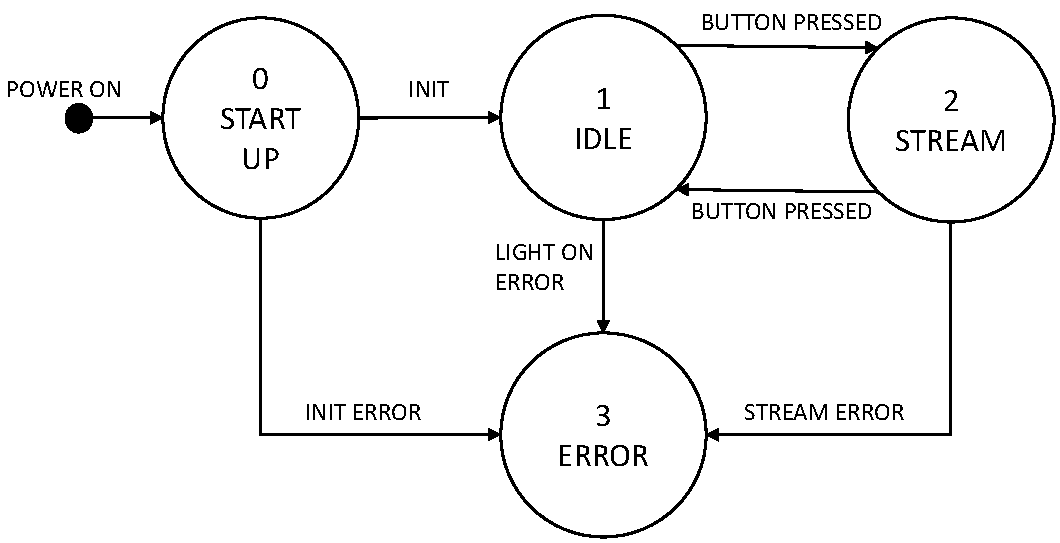
\includegraphics[width=0.6\linewidth]{ImageFiles/Macchina a stati finiti/FSM}
	\caption{Macchina a stati finiti del firmware delle due board progettate.}
	\label{fig:FSM}
\end{figure}

\paragraph{Start-up}
Lo stato di \textit{Start-up} rappresenta la fase di inizializzazione del sistema. Quando la board STM32F4DISCOVERY viene alimentata tramite una porta usb, il microcontrollore si avvia e entra nello stato di \textit{Start-up}. Ad ogni condizione del sistema è stata associata ad un indicatore luminoso (uno dei quattro LED integrati sulla board) per segnalare all'utente lo stato attivo. Mentre il sistema si trova nello stato \textit{Start-up} il LED arancio rimane acceso. Vengono inizialmente configurate tutte le periferiche necessarie al funzionamento della comunicazione I\ap{2}C, della porta seriale USB e vengono inizializzati i pin della GPIO. Inoltre, sono inizializzate anche le strutture necessarie alle librerie HAL, presentate nella sezione~\ref{sec:Firmware}, fondamentali per la comunicazione I\ap{2}C. Di seguito, viene effettuata la lettura tramite I\ap{2}C del registro del sensore PPG che contenente il \textit{part-id} della scheda. Se non ci sono errori di lettura e l'identificativo acquisito rispetta le informazioni contenute nel datasheet del sensore, si può proseguire con l'inizializzazione della struttura dati che conterrà tutte le informazioni per la configurazione del sensore. Nel caso di errore, il sistema andrà nello stato di \textit{Error}. A questo punto, vengono scritti i registri che determinano la configurazione del modulo PPG. Se l'operazione di scrittura avviene correttamente, il sistema può transitare nello stato di \textit{Idle}, altrimenti entra nello stato di \textit{Error}.
\paragraph{Idle} 
\paragraph{Stream}
\paragraph{Error}

\clearpage